\section{Анализ полученных данных}
\label{sec:analysis}

В данной описывается влияние параметров системы на сжатие изображений.
Параметры влияние которых исследовалось:

\begin{itemize}
  \item частота дискретизации;
  \item количество входных нейронов сети;
  \item количество нейронов на самом узком участке нейронной сети;
  \item количество тестовых примеров, подобранных для обучения сети.
\end{itemize}

В итоге был сформирован такой набор тестов:

\begin{itemize}
  \item 3 глубины дискретизации изображения(8,32 и 256 уровней);
  \item 4 множества входных нейронов сети(16, 25, 64 и 100 нейронов);
  \item 6 отношений количества нейронов на самом узком участке сети к количеству входных нейронов(2 к 8, 3 к 8, 4 к 8, 5 к 8, 6 к 8 и 7 к 8);
  \item 15 наборов тестов к каждому обучению сети в количестве от 10 до 150 с шагом 10.
\end{itemize}

Было проведено 7560 тестов. Процесс был расспараллен на все вычислительные потоки центрального процессора.
Каждый поток обрабатывал тесты для одного изображения и сохранял данные о результатах тестирования в тектовый файл,
но вычисления все равно заняли 5 суток процессорного времени.
Программа собирала данные о времени затраченном на сжатие изображения в конкретном тесте, степень сжатия,
соотношение сигнал-шум и среднеквадратическое отклонение для исходного и полученного изображения.
Так же программа сохраняла изображение в сжатом виде и его декодированную версию.

\subsection{Частота дискретизации}
\label{sub:analysis:discrete}

\begin{figure}[ht]
\centering
  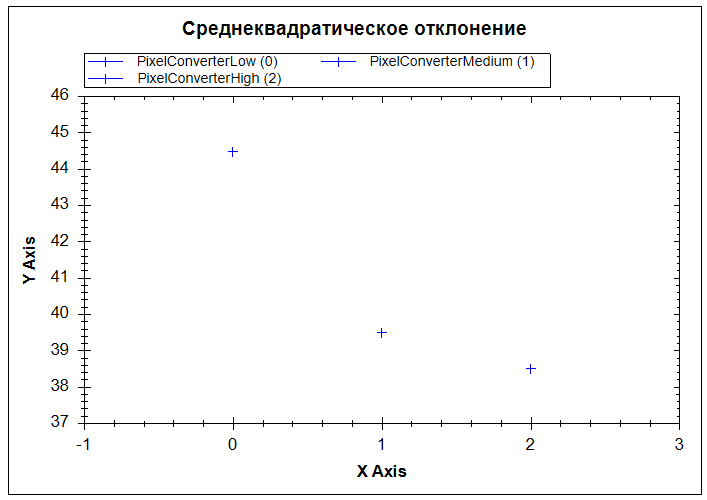
\includegraphics[scale=0.5]{ByConverterMSC.png}
  \caption{ зависимость значений среднеквадратичного отклонения от глубины дискретизации }
  \label{fig:by_converter_msc}
\end{figure}

\begin{figure}[ht]
\centering
  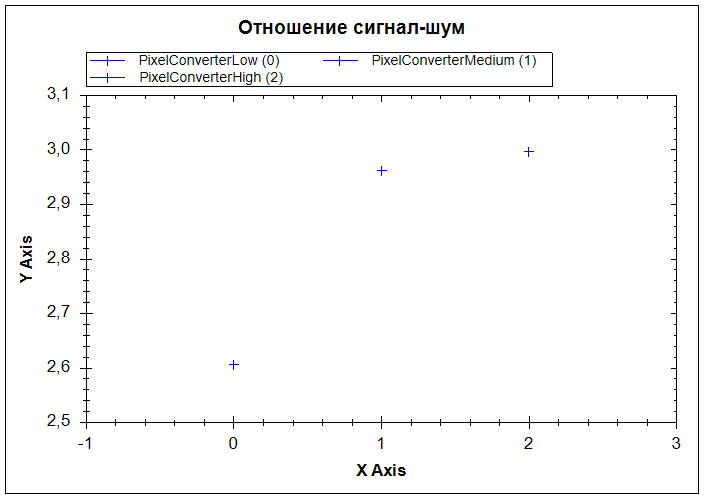
\includegraphics[scale=0.5]{ByConverterSNR.png}
  \caption{ зависимость значений отношения сигнал-шум от глубины дискретизации }
  \label{fig:by_converter_snr}
\end{figure}

\begin{figure}[ht]
\centering
  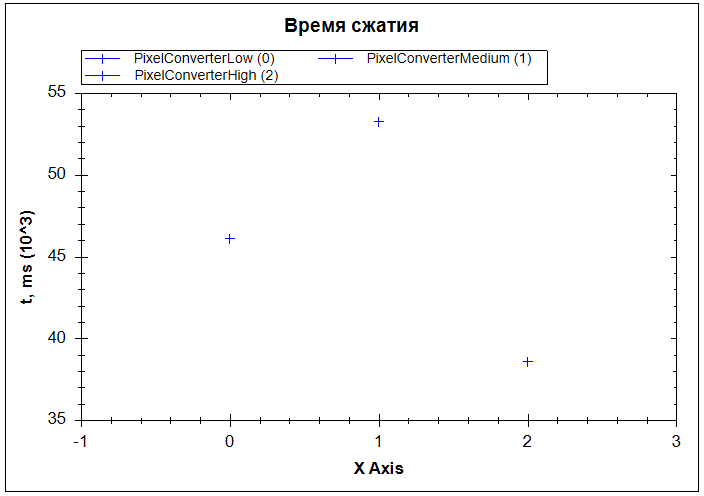
\includegraphics[scale=0.5]{ByConverterBuildTime.png}
  \caption{ зависимость времени сжатия от глубины дискретизации }
  \label{fig:by_converter_build_time}
\end{figure}

\begin{figure}[ht]
\centering
  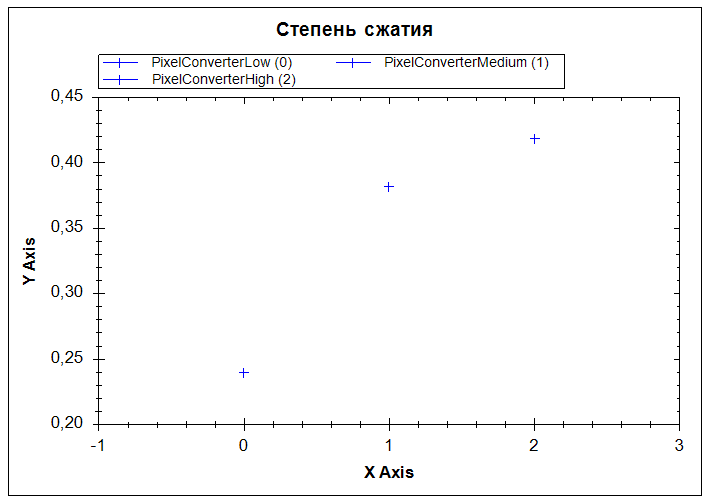
\includegraphics[scale=0.5]{ByConverterSize.png}
  \caption{ зависимость отношения итогового размера к исходному размеру от глубины дискретизации }
  \label{fig:by_converter_build_time}
\end{figure}

\subsection{Размер входного блока}
\label{sub:analysis:input}

\begin{figure}[ht]
\centering
  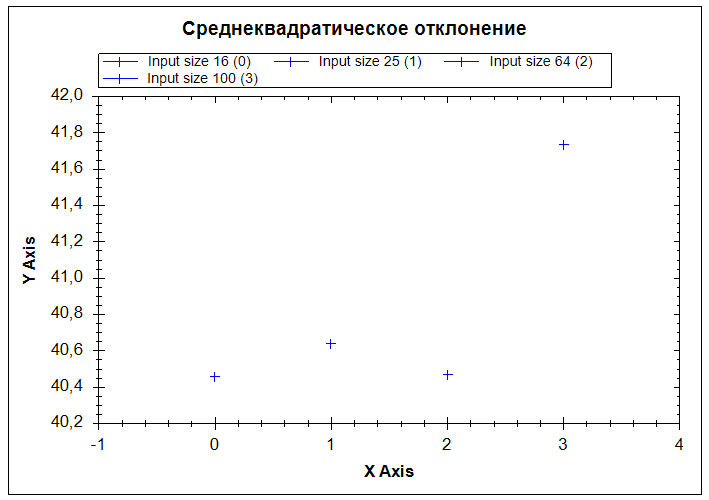
\includegraphics[scale=0.5]{ByInputMSC.png}
  \caption{ зависимость значений среднеквадратичного отклонения от количества нейроннов на входном слое }
  \label{fig:by_input_msc}
\end{figure}

\begin{figure}[ht]
\centering
  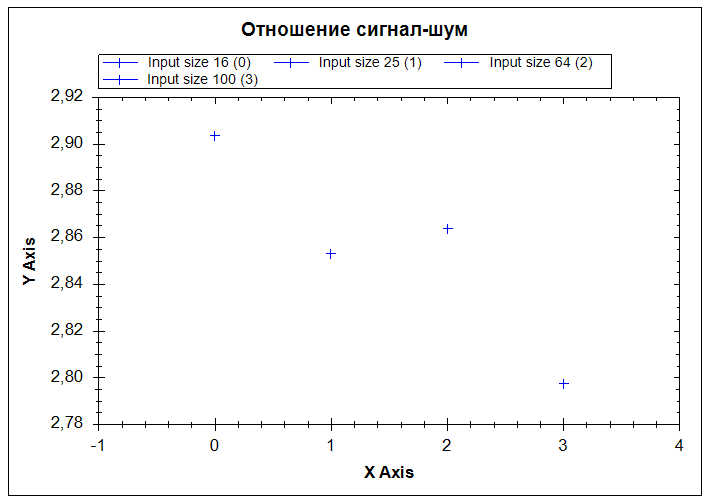
\includegraphics[scale=0.5]{ByInputSNR.png}
  \caption{ зависимость значений отношения сигнал-шум от количества нейроннов на входном слое }
  \label{fig:by_input_snr}
\end{figure}

\begin{figure}[ht]
\centering
  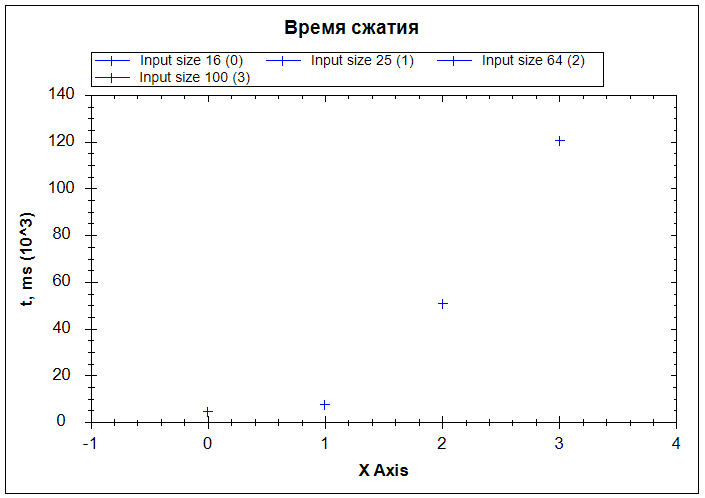
\includegraphics[scale=0.5]{ByInputBuildTime.png}
  \caption{ зависимость времени сжатия от количества нейроннов на входном слое }
  \label{fig:by_input_build_time}
\end{figure}

\begin{figure}[ht]
\centering
  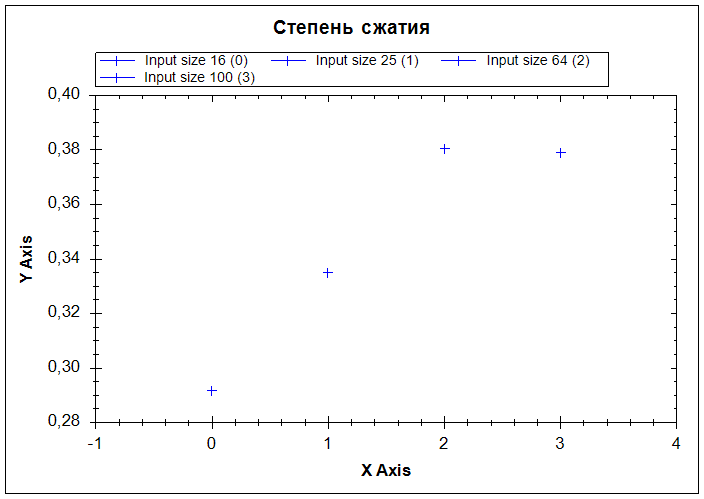
\includegraphics[scale=0.5]{ByInputSize.png}
  \caption{ зависимость отношения итогового размера к исходному размеру от количества нейроннов на входном слое }
  \label{fig:by_input_build_time}
\end{figure}

\subsection{Соотношение количества нейронов между слоями}
\label{sub:analysis:output}

\begin{figure}[ht]
\centering
  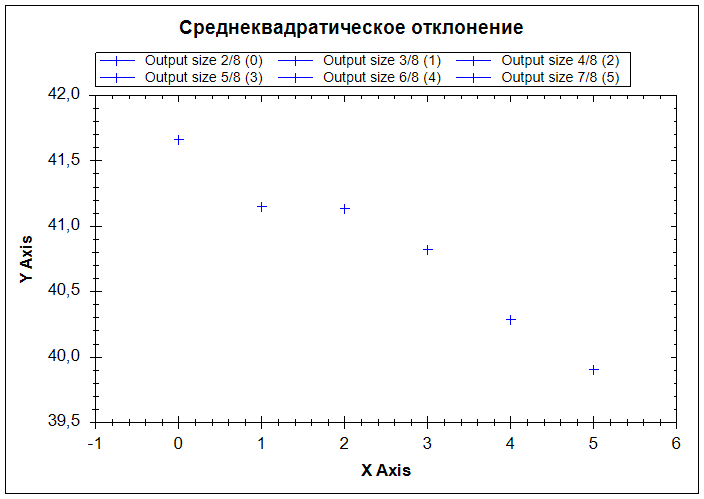
\includegraphics[scale=0.5]{ByOutputMSC.png}
  \caption{ зависимость значений среднеквадратичного отклонения от отношений количества нейронов на слоях }
  \label{fig:by_output_msc}
\end{figure}

\begin{figure}[ht]
\centering
  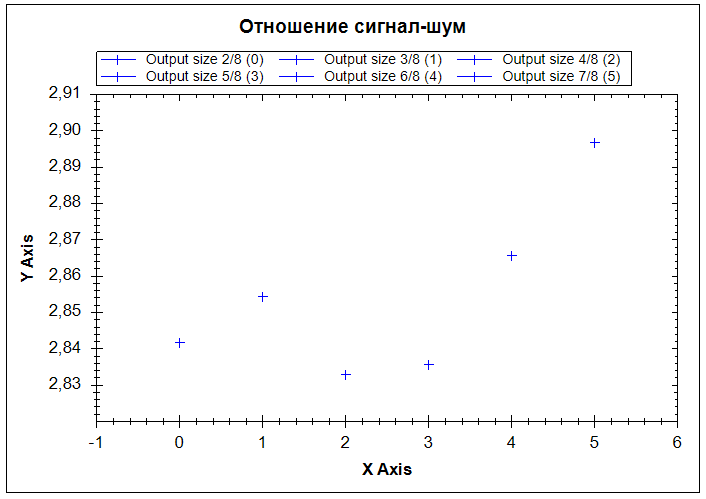
\includegraphics[scale=0.5]{ByOutputSNR.png}
  \caption{ зависимость значений отношения сигнал-шум от отношений количества нейронов на слоях }
  \label{fig:by_output_snr}
\end{figure}

\begin{figure}[ht]
\centering
  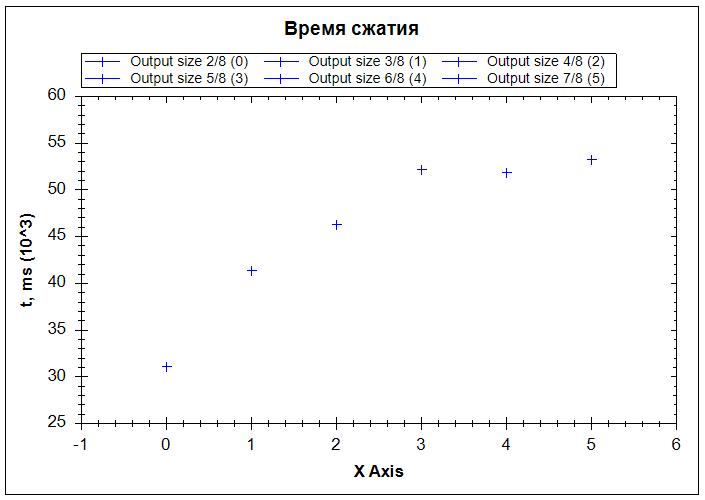
\includegraphics[scale=0.5]{ByOutputBuildTime.png}
  \caption{ зависимость времени сжатия от отношений количества нейронов на слоях }
  \label{fig:by_output_build_time}
\end{figure}

\begin{figure}[ht]
\centering
  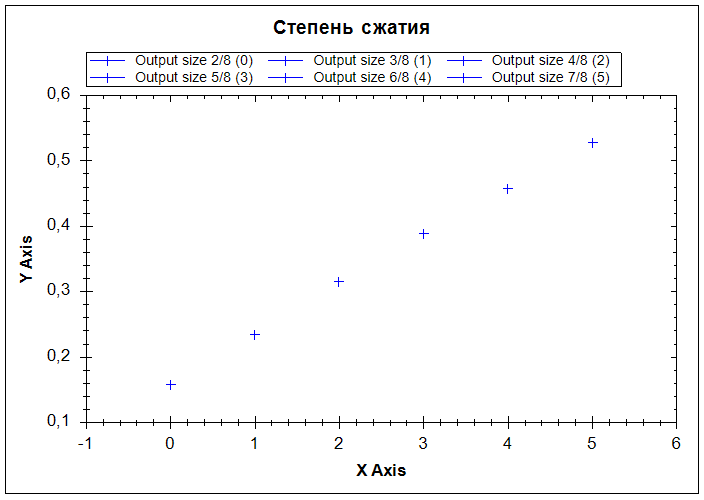
\includegraphics[scale=0.5]{ByOutputSize.png}
  \caption{ зависимость отношения итогового размера к исходному размеру от отношений количества нейронов на слоях }
  \label{fig:by_output_build_time}
\end{figure}

\subsection{Количество тестов для обучения нейронной сети}
\label{sub:analysis:tests}

\begin{figure}[ht]
\centering
  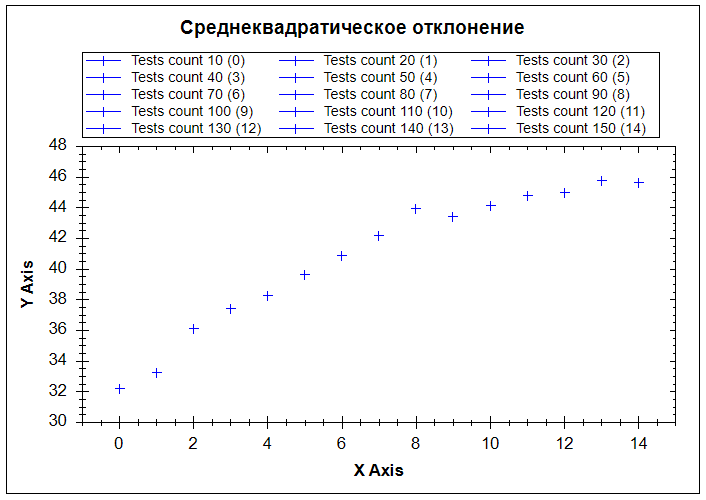
\includegraphics[scale=0.5]{ByTestsCountMSC.png}
  \caption{ зависимость значений среднеквадратичного отклонения от размера данных для обучения нейронной сети }
  \label{fig:by_tests_count_msc}
\end{figure}

\begin{figure}[ht]
\centering
  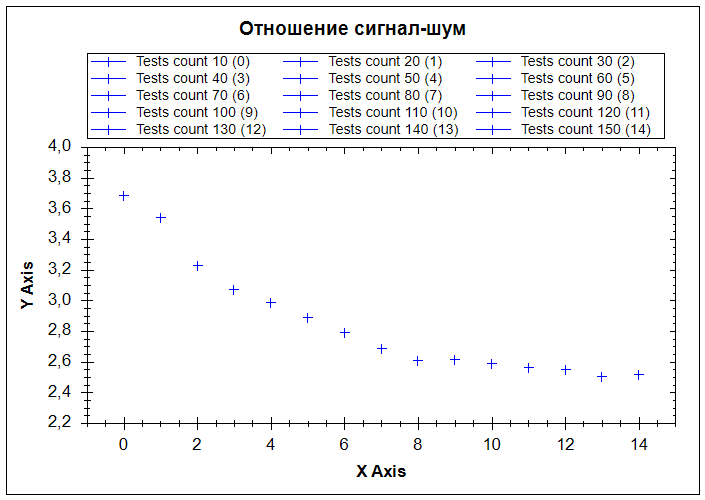
\includegraphics[scale=0.5]{ByTestsCountSNR.png}
  \caption{ зависимость значений отношения сигнал-шум от размера данных для обучения нейронной сети }
  \label{fig:by_tests_count_snr}
\end{figure}

\begin{figure}[ht]
\centering
  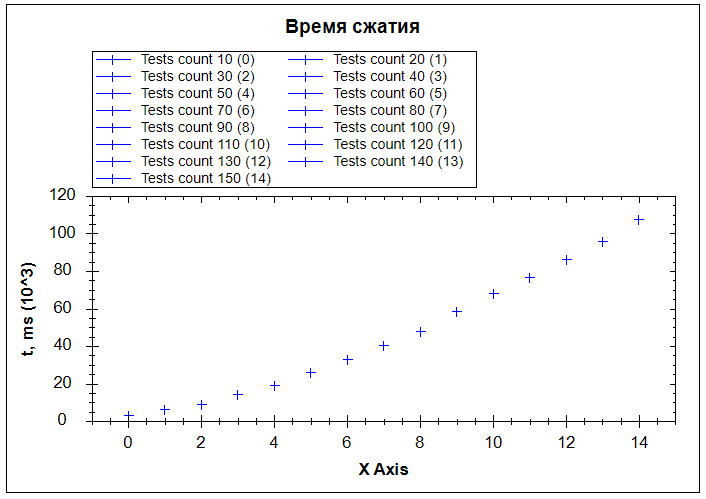
\includegraphics[scale=0.5]{ByTestsCountBuildTime.png}
  \caption{ зависимость времени сжатия от размера данных для обучения нейронной сети }
  \label{fig:by_tests_count_build_time}
\end{figure}

\begin{figure}[ht]
\centering
  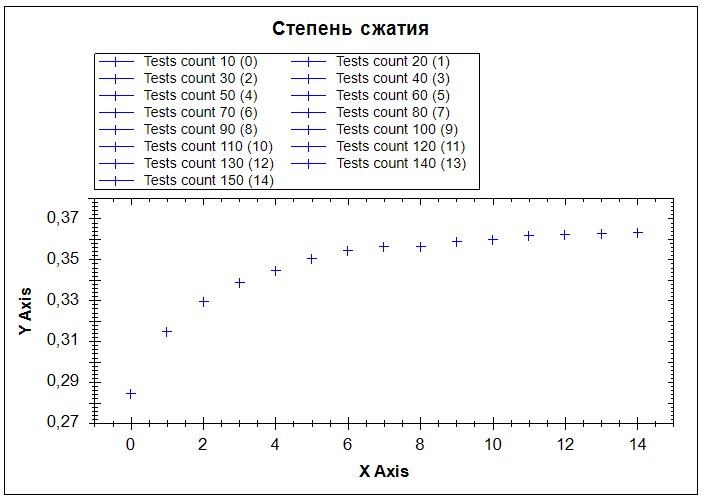
\includegraphics[scale=0.5]{ByTestsCountSize.png}
  \caption{ зависимость отношения итогового размера к исходному размеру от размера данных для обучения нейронной сети }
  \label{fig:by_tests_count_build_time}
\end{figure}
